\begin{checkit}
This work will be reported in \emph{Paul et al., 2019, Experimental Astronomy}. I would like to sincerely thank Professor A R Rao, my PhD advisor, for giving me the opportunity for doing this work, and the permission to use the L2 CZTI data for a number of sources as and when required; Professor Dipankar Bhattacharya in IUCAA [Pune, India] for encouragement and support throughout the course of the work; Mithun NPS in PRL [Ahmedabad, India] for his extremely helpful suggestions at crucial stages of the work, as well as long discussions clarifying doubts regarding the existing pipeline and its data files. Last but not the least, all the data used in the work were kindly made available by the CZTI-POC [Payload Operation Centre] in IUCAA [Pune, India], all queries regarding which were timely attended by the people there, to whom collectively I extend sincere thanks.
\end{checkit}



\section{Introduction}
\label{sec:introduction--noise}
In Chapters \ref{chap:LGRBs} and \ref{chap:SGRBs}, it was shown that \AS -CZTI misses out on a number of GRBs, both long [Section \ref{subsec:predictions_for_CZTI--long}] and short [Section \ref{subsec:predictions_for_CZTI--short}]. The reasons are investigated in this chapter via a thorough re-look at the data analysis pipeline in place for CZTI.

In the CZTI terminology, an `event' is a trigger of any of the pixels, associated with an unique time-stamp, the pixel co-ordinates, and the `pulse height amplitude' or PHA, which is linearly related to the energy of the photons that triggered the pixel. Being a wide-field open detector, CZTI detects photons from all directions within its wide FOV. These photons include those from the target source, called `science' events, as well as those induced by other sources. The latter can include a steady rate of events induced by the charged particle environment of the detector, which other than showing predictable variation with the satellite co-ordinates, should show uniform random distribution about the mean. These events are called `background' events. On top  of this, events may be generated by the peculiarities in the detector and may not be triggered by photons in the first place. These need to be identified and removed before doing any scientific investigation of the events from the target source both in the temporal and energy domains, and are called `noise' events. Only a careful analysis of the data can precisely define characteristics of noise, and subsequently eliminate them for the study of the science data.

The presence of cosmic ray induced noise events was deduced during the first days of the mission, and a simple algorithm implemented in the existing CZTI pipeline to eliminate them from the science data. They are easily distinguished from science events due to the temporal characteristics: they all `bunch' together within the smallest interval of time resolvable by the CZT pixels, $20 \, \mus$ \citep{Bhalerao_et_al.-2017-JApA}. A steady stream of these `bunches' triggered by cosmic rays continuously bombard the detector plane. They temporally track the variation of the cosmic rays bombarding the entire satellite, independently measured by the Charged Particle Monitor [CPM] on-board \AS\ \citep{Rao_et_al.-2017-JApA}.

In this work, we have conducted a careful analysis of the data collected by CZTI for a number of GRBs. It is shown via careful reasoning that improvements in our understanding of bunches can be made. `Double-events' are those that occur on neighbouring pixels at the same time [i.e. within $20 \, \mus$], and are used for polarization measurements by CZTI \citep{Chattopadhyay_et_al.-2014-ExA, Chattopadhyay_et_al.-2017-arXiv}. The effect of electronic noise on double-events is quantified by studying the behaviour of the bunched events during GRBs. Moreover, identification of heavy deposition of charge by very high energetic particles is done via patterns on the detector modules that are characteristic of pixelated detectors collecting data at such high time resolutions. A new algorithm is developed which automatically identifies and removes these events from the data to create further cleaned science data.

The software has been tested in the \textsc{python} programming language. The scripts have being made publicly available at: \url{https://github.com/DebduttaPaul/useful_functions_for_CZTI_data_analysis}. The effects of of cosmic rays via bunches are carefully reinvestigated in Section \ref{sec:Bunchclean}, suggesting improvements of the current data flow in the existing CZTI pipeline. The effect of these `bunched' events on genuine events are quantified. In Section \ref{sec:Gross_noisy_pixels}, the flagging of grossly noisy elements are re-examined. In Section \ref{sec:DPHclean}, the effect of higher energetic cosmic rays on the CZTI data are reported, via an algorithm detailed in Appendix \ref{appendix:DPHstructures}. In Section \ref{sec:conclusions--noise}, concluding remarks are presented.


\section{Re-look at `cztbunchclean'}
\label{sec:Bunchclean}
The overall instrument configuration, the detectors and electronics, the data characteristics, processing pipeline and default products have been discussed in detail in \cite{Bhalerao_et_al.-2017-JApA}. All the work carried out in this chapter uses the astronomer-friendly `Level 2' [L2] FITS files created by the Payload Operation Centre [POC] of CZTI, located in the Inter-University Centre for Astronomy \& Astrophysics [IUCAA] in Pune, India. This is executed by the first task in the CZT pipeline\footnote{\url{http://astrosat-ssc.iucaa.in/uploads/czti/CZTI_level2_software_userguide_V2.1.pdf}}: the  \textbf{cztscience2event}. The on-board bunchclean identifies the bunches present in the data, and removes the events except three events at the boundaries of each bunch for the purpose of latter identification; more details can be found in the above document. The next task in the pipeline is \textbf{cztbunchclean}, which removes the bunched events in the data remnant after the onboard bunchclean. In addition, currently it removes data for certain lengths of time \emph{skipT1}, \emph{skipT2}, \emph{skipT3} after the bunches, depending on the number of events in the bunch, termed as \emph{bunch\_length\_threshold}. The values for these parameters have been set somewhat arbitrarily. In this section, we take a re-look at this task, and suggest alternatives to the parameters in the existing pipeline. For this, we have additionally used the data in the bunch files created by \textbf{cztscience2event}, to be henceforth termed as `bunch-files'.

\subsection{Redefining bunches}
\label{subsec:redefining_bunches}
The understanding behind the idea of bunches is that each bunch is created by one cosmic ray particle generating a series of electronic events within timescales shorter than the instrumental resolution of $20 \, \mus$. If such is the case, then respective bunches are independent of each other, and the interval between one bunch and the next, $\Delta T$, is expected to follow a smooth distribution. On plotting the histogram of $\Delta T$ by using the bunch data, it is clearly seen that such is not the case, see \eL\ of Figure \ref{fig:bunch_redefinition}. This leads one to assume that the electronic effects of a single charged particle lasts for more than the time-resolution of the instrument. Hence we propose to redefine bunches such that, if the interval between one bunch and the next is less than a certain threshold $t_2$, then these two bunches are understood to be created by the same cosmic ray particle and all the data within it are clubbed to a single bunch, henceforth termed a `super-bunch'. Empirically, it is seen that the sharp spike is removed on choosing $t_2 = 60 \, \mus$. For $t_2 = 40 \, \mus$, the spike is still clearly visible, whereas for $t_2 = 80 \mus$, the spike is replaced by a dip, clearly showing that it is an overkill. Thus, $60 \, \mus$ is optimal, see \eR\ of Figure \ref{fig:bunch_redefinition}. It is observed that less than $10 \%$ bunches are redefined as `super-bunches'.

\begin{figure}
\begin{center}
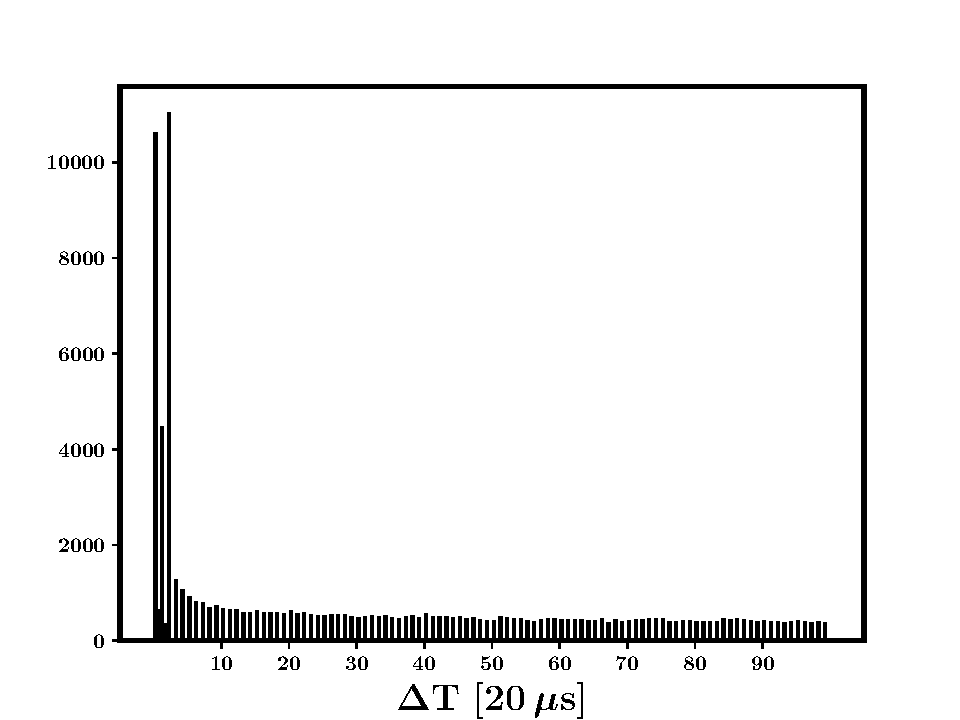
\includegraphics[scale=0.42]{GRB160802A--Q3--Interval_between_Bunches_Histogram--raw_data}
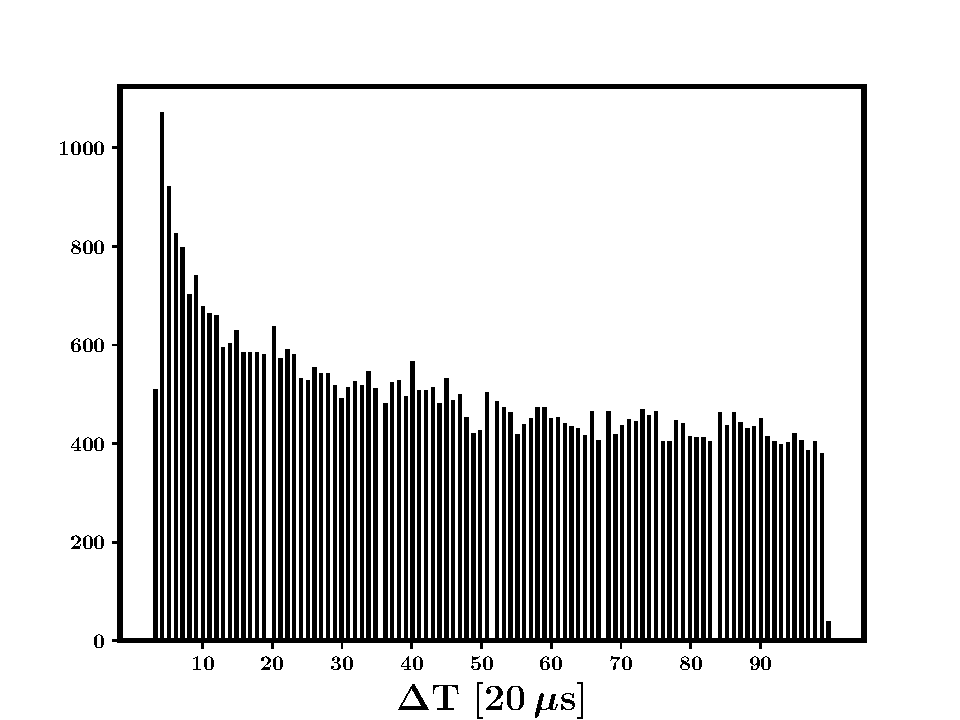
\includegraphics[scale=0.42]{GRB160802A--Q3--Interval_between_Bunches_Histogram--after_bunch_redefinition}
\caption[The re-definition of bunches]{$\Delta T$ is defined as the time interval between the end of a bunch and the start of the next bunch. \eL: Bunch data after \textbf{cztscience2event}. The histogram peaks at small $\Delta T$ clearly showing that the definition of bunches is incorrect. The parameter for bunch redefinition, such that the histogram becomes smooth is referred to as $t_2$. \eR: With $t_2 = 60 \, \mus$, the histogram indeed becomes smooth. Although the above plots are taken from one orbit of March background data, this observation is true for all datasets examined. The first point in corresponds to the bunch redefinition timescale, and is an artefact created due to the limitation of the way division is carried out in the binary system; it persists whatever value of $t_2$ is used, but is unimportant for our purposes.}
\label{fig:bunch_redefinition}
\end{center}
\end{figure}

\subsection{Post-bunch cleaning}
\label{subsec:post-bunch_clean}

\begin{figure}
\begin{center}
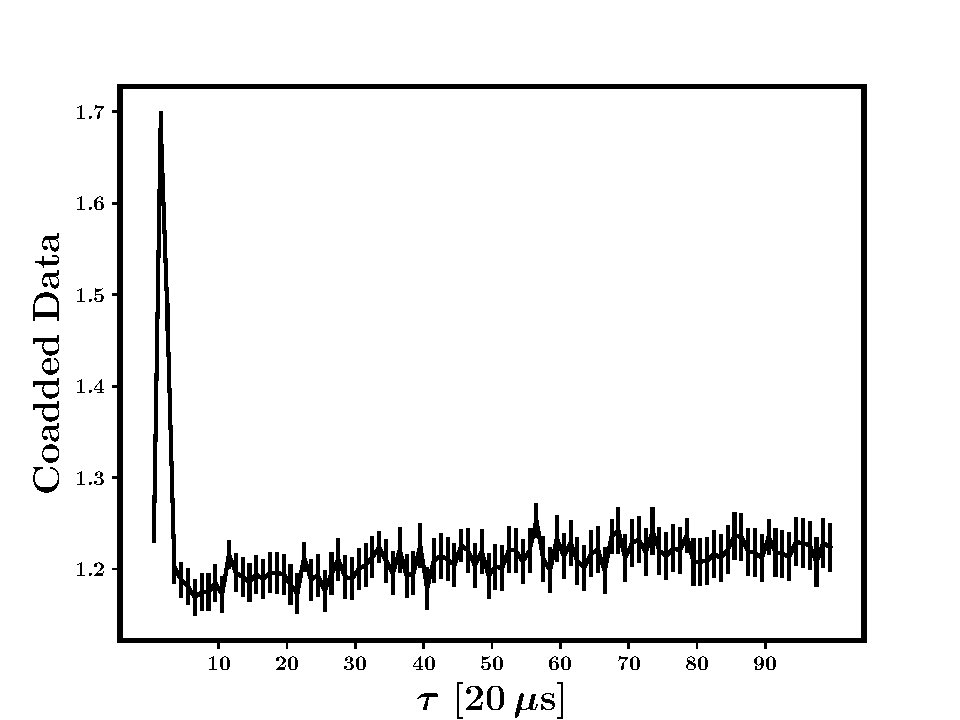
\includegraphics[scale=0.42]{GRB160802A--Q1--LC--raw_data}
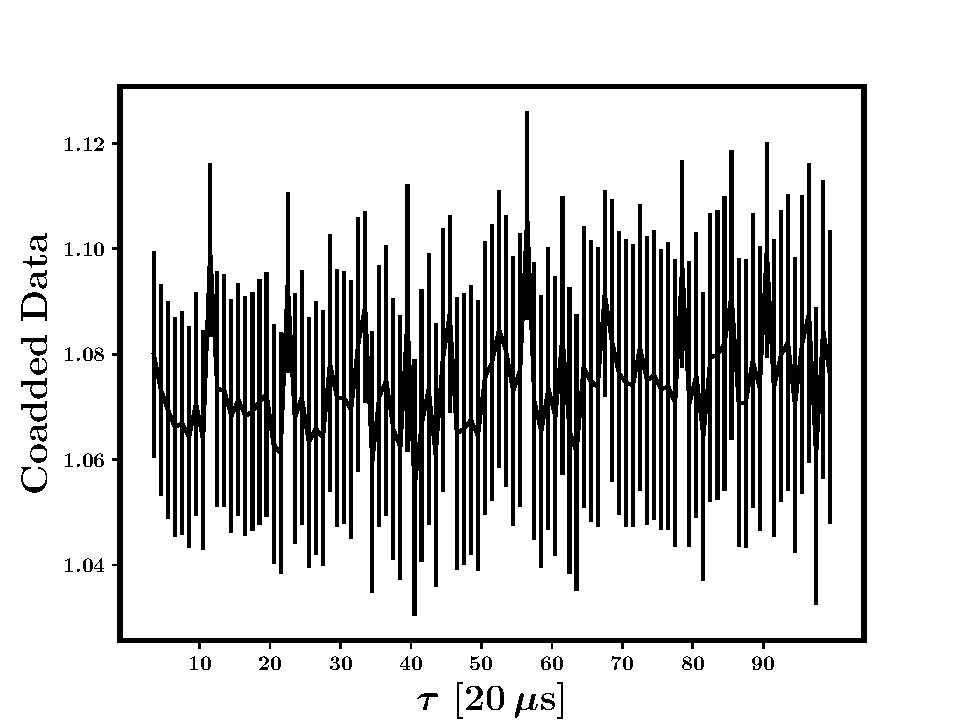
\includegraphics[scale=0.42]{GRB160802A--Q1--LC--after_new_bunchclean}
\caption[The remnant effect of \textbf{cztbunchclean}]{\eL: A sharp drop is seen at timescales lesser than $60 \, \mus$ if co-added lightcurve, corrected for the exposure, is made from data post bunches, even after redefining bunches. This implies that post bunches, significant amount of electronic noise, created by the bunches, is persistent. Hence, data post bunches is removed up to the parameter $t_3$. \eR: After flagging \emph{all} data post bunches, with $t_3 = 60 \, \mus$, the co-added lightcurve looks flat as expected, all the way up to $2$ ms, validating the assumption. All errors assume that the data is Poissonian, which is strictly true for the part away from the spike in \eL.}
\label{fig:postbunch_flagging}
\end{center}
\end{figure}


As noticed earlier, the electronic effects of cosmic-ray particles persist for some amount of time post-bunch, after initially triggering a series of events in the detector. We parametrize this timescale  as $t_3$, similar to \emph{skipT1}, \emph{skipT2}, \emph{skipT3}. To estimate the optimum value of $t_3$, we plot co-added lightcurves of events after the bunches. That is, we choose only the data from the end of each bunch to the next bunch, including the superbunches defined in Section \ref{subsec:redefining_bunches}, define the end of the bunches as $t = 0$, order the dataset thus formed from all the bunches, and then add these datasets. Shown in Figure \ref{fig:postbunch_flagging} is the ratio of this co-added data to the total exposure, where the exposure for each bunch is defined as the total number of instances that data is available between the chosen bunch and the next. This ratio is chosen to remove the overall Poissonian trend of the co-added data with time, and look for any remnant effects. If the data is fully Poissonian, then it should vary randomly about unity, for all times. In the \eL\ of the Figure, we see a sharp rise and fall at the smallest of $t$, which is indicative of remnant electronic effects even after redefining the bunches as described in Section \ref{subsec:redefining_bunches}.

We experiment with different values of $t_3$. On choosing  $t_3 = 60 \, \mus$ and removing data for $t_3$ after each bunch [including superbunches], the co-added lightcurve indeed becomes flat around unity, implying that the removal of cosmic ray induced noise is finally complete. \eR\ of Figure \ref{fig:postbunch_flagging} demonstrates this.

We have re-examined whether flagging only the affected detector modules also give the same result. For this we used long stretches of the same data, and experimented with different values of \emph{bunch\_length\_threshold} to check whether heavier bunches affect nearby detector modules as well. It is found that that there is no difference to the resulting cleaned data if selective cleaning is done to only affected detector modules or not, based on \emph{bunch\_length\_threshold}. The optimized value of $t_3$ is so small that most of the data successive to the bunches are mostly in the same modules, hence no difference is made. Thus, instead of three parameters for post bunch cleaning, only one is sufficient. $t_2 \sim t_3$ leads one to assume that the physical mechanism behind both the effects are same, that is electronic noise in the hardware, which is quantified in the next subsection.

The newly proposed method of cleaning the L2 data of bunches, constituting the two steps demonstrated in Section \ref{subsec:redefining_bunches} and \ref{subsec:post-bunch_clean}, is to be henceforth collectively and simply called `bunchclean', as against `on-board bunchclean' which leaves three events from each bunch in the dataset, and the pipeline task \textbf{cztbunchclean} which invokes the usage of the parameters \emph{skipT1}, \emph{skipT2}, \emph{skipT3}, \emph{bunch\_length\_threshold}.


\subsection{Using bunches to quantify electronic noise created by source photons}
\label{subsec:electronic_effects}

We have carried out a preliminary examination of lightcurves of bunches for a few datasets, i.e. the time-series of the number of bunches detected, see Figure \ref{fig:bunch_enhancement_during_bright_GRBs} for an example. Sudden increase of the bunch-rate lasting for a few seconds are seen in such lightcurves, corresponding to possible increase of cosmic ray induced events. These features appear randomly in different datasets and quadrants. Moreover, they are almost always due to bunches with bunch-length [total number of events constituting a bunch] equal to $3$ instead of higher. Sometimes bunches of greater lengths show gradual increase from the continuum level, but these features are not as sharp; moreover, they appear uncorrelated to bunches of length $3$.

Temporal features in the bunches lasting for $\gtrsim 10$ s always appear at the same instances for bunches of different lengths. These are extremely rare [$\sim$ once in $10$ orbits of data] phenomenon, and seem to affect Q3 the most, followed by Q2; however this statement is subject to low-count statistics. If it is true on the other hand, it can be understood to be caused by the fact that these quadrants are in the open side of the satellite and is hence prone to high energetic charged particles: Q3 is open from two sides as compared to one for Q2, wheres Q0 and Q1 are closed by high-Z absorbers from all sides.

\begin{figure}
\begin{center}
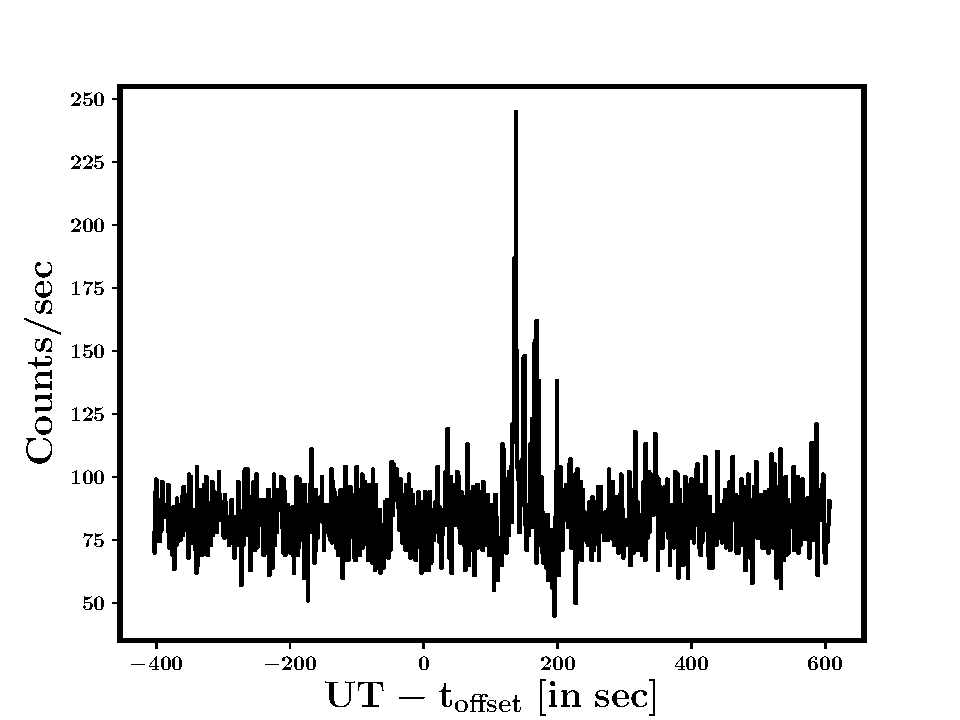
\includegraphics[scale=0.42]{GRB160821A--Q1--all_bunch_LC--1s}
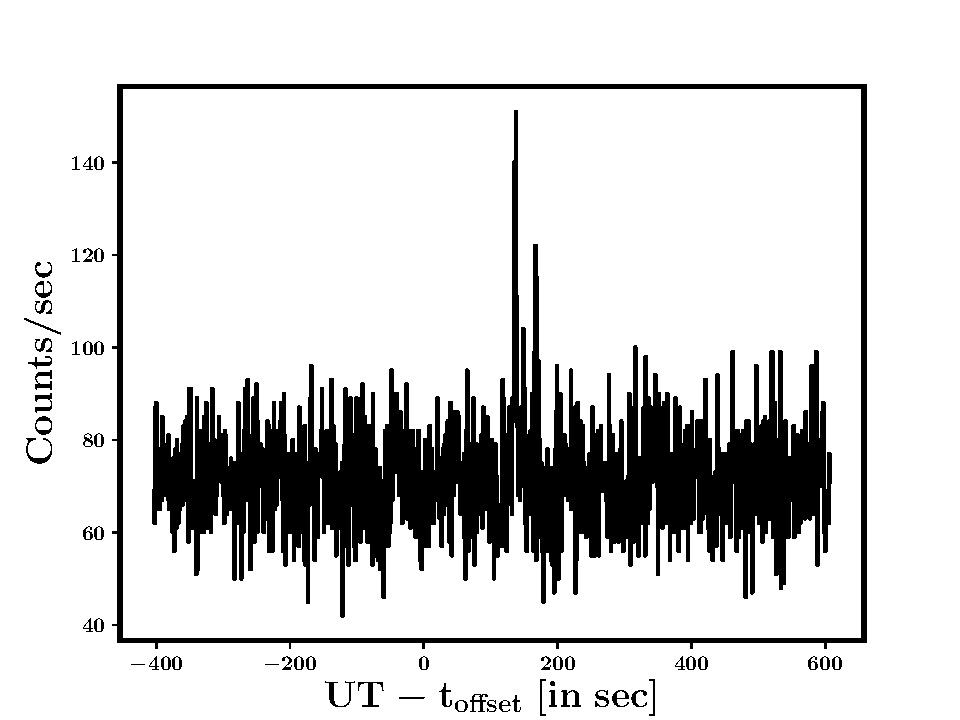
\includegraphics[scale=0.42]{GRB160821A--Q1--Tg_bunch_LC--1s}
\caption[Enhancement of number of bunches during bright GRBs]{Bunch lightcurves for bright GRB160821A, with the time axis offset to the known GRB trigger time [note that the trigger time in all quadrants of CZT data as well as Veto for this GRB is offset by $\sim 150$ s from the value reported by IceCube]. Such an enhancement is not expected if all bunches are due to cosmic rays. \eL: All bunches. \eR: Bunches with total number of events greater than $3$ also show enhancement. Increasing this threshold does not suppress this effect, implying that GRB photons trigger electronic events mimicking as short as well as bunches.}
\label{fig:bunch_enhancement_during_bright_GRBs}
\end{center}
\end{figure}


If bunches are all indeed created by cosmic ray photons, then they should not show any enhancement during GRBs. Figure \ref{fig:bunch_enhancement_during_bright_GRBs} demonstrates that bunches do exhibit such an unexpected enhancement, although this phenomenon is extremely rare, seen for only the brightest of GRBs, e.g. GRB160623A, GRB160802A, GRB160821A. During these bright flashes, the chance-coincidence of single events with others may mimic double-events, and similarly, their chance-coincidence with double-events may mimic bunches. Let us denote the average single-event rate as $r_{\rm{1,b}} \sim 200 \, \ps$, the average double-event rate as $r_{\rm{2,b}} \sim 70 \, \ps$ etc., the temporal resolution of CZTI as $\delta t =  20 \, \mus$, and the excess single-event rate during a bright GRB as $r_1 \sim 2000 \, \ps$. Then the chance-coincidence production rate of double-events during a GRB is $r_{\rm{1}} r_{\rm{1,b}} \delta t = 8 \, \ps$, and the chance-coincidence production rate of bunches is $r_{\rm{1}} r_{\rm{2,b}} \delta t = 2.8 \, \ps$. The chance-production rate of higher length bunches will be even smaller, and hence can be neglected. Thus, we see that only chance-coincidence cannot explain the enhancement of bunches during bright GRBs, falling short by at least one order of magnitude. Hence the identification of all bunches with cosmic rays is questionable. Moreover, the enhancement correlates with the GRB flux, being $\sim 80 \, \ps$ for GRB160623A, GRB160802A and $\sim 150 \, \ps$ for GRB160821A, the latter being brighter than the former two by roughly the same factor. We attempted to segregate this effect into bunches of different lengths, i.e. examined that whether the enhancement of the bunch-rate is only for bunches lesser than a certain length. Although the enhancement during the GRBs is progressively lesser for bunches of higher lengths, for GRB160821A the enhancement is clearly seen for bunch lengths at least up to $6$ [see \eR\ of Figure \ref{fig:bunch_enhancement_during_bright_GRBs}].

\begin{figure}
\begin{center}
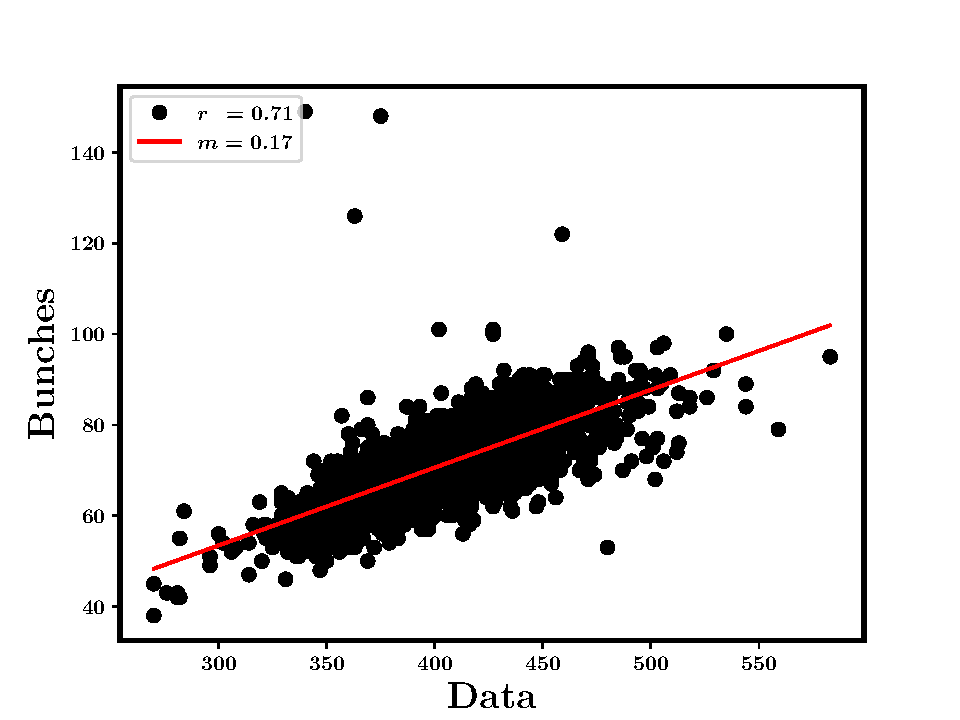
\includegraphics[scale=0.42]{GRB160821A--BKG_fit}
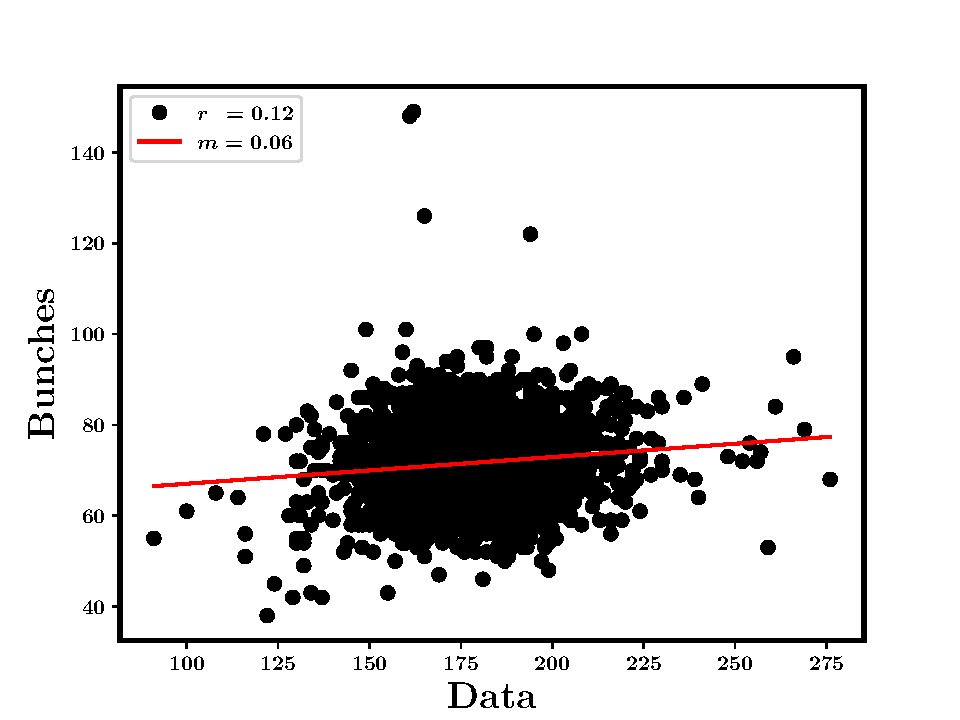
\includegraphics[scale=0.42]{GRB160821A--BKG_fit--with_Bunchclean}
\end{center}
\begin{center}
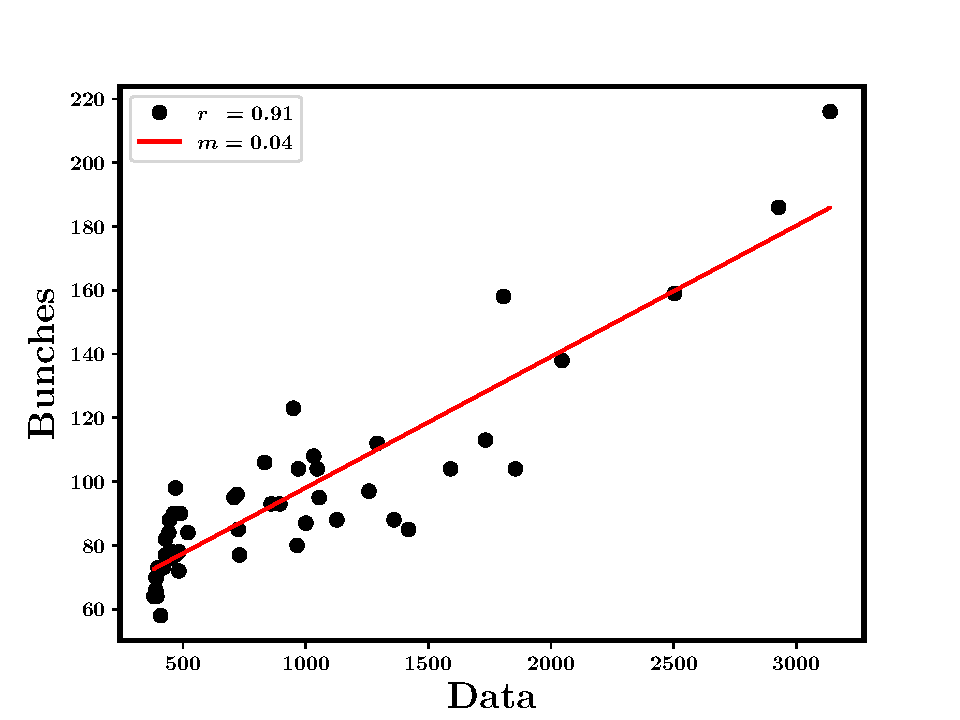
\includegraphics[scale=0.4]{GRB160802A--GRB_fit}
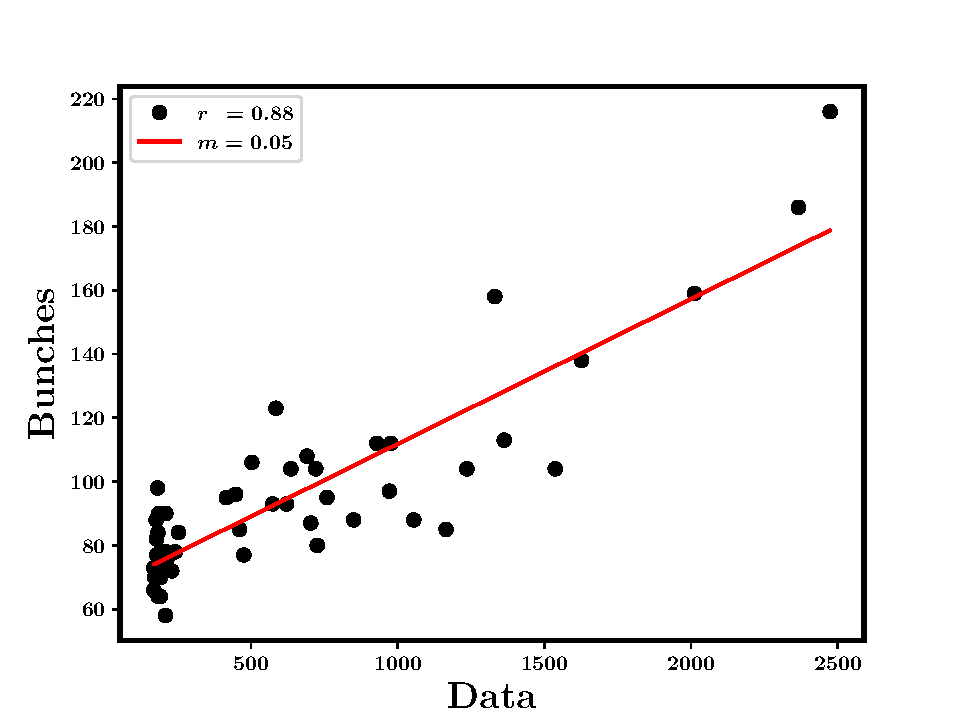
\includegraphics[scale=0.4]{GRB160802A--GRB_fit--with_Bunchclean}
\caption[Correlation between bunch-rate and event-rate]{\emph{Top}: Bunch-rate versus event-rate [corrected for livetime] away from the duration of the very bright GRB160821A. $r$ is the Pearson correlation coefficient, $m$ is the slope of the fitted straight line. \eL: In the raw data including bunches, i.e. before bunchclean. \eR: After bunchclean: the correlation is gone, and the scale in the x-axis is reduced by half. The slope is reduced by a factor of $\sim 3$. \emph{Bottom}: During the duration of the bright GRB160802A. \eL: Before bunchclean. \eR: After bunchclean; the correlation is still present. It is primarily driven by the small number of bins corresponding to the GRB excess. The slope obtained is comparable for all the three bright GRBs examined, before as well as after bunchclean. This clearly proves that there is a driving mechanism of the bunch excess by the GRB excess, independent of datasets used or the duration or flux of the GRBs. The similarity in the slope with that of the data devoid of GRBs post cleaning [\emph{Top-Right}] is also indicative of the universality of this driving mechanism, implying that \emph{all} source photons, including sky background, create such an electronic effect. Not all bunches can hence be thought to cosmic ray triggered. However, this gives an overall scaling in the number of bunches as well as double events. All bunches, whether induced by cosmic rays or this electronic mechanism, need to be removed anyway.}
\label{fig:correlations}
\end{center}
\end{figure}


The bright GRBs provide the opportunity to study electronic effects that remain otherwise hidden in the data. For these GRBs, we create time-series of the total data, as well as the number of bunches, binned at the same timescale. Then we plot these two time-series data against each other, shown in Figure \ref{fig:correlations}. First we consider time intervals that do not include the GRBs. A clear correlation is seen between the two time series. However, the correlation vanishes on executing `bunchclean'. The correlation, and its absence on implementing bunchclean on the dataset, is simply due to the fact that the overall event-rate depends on the cosmic ray induced events. This becomes clear by considering the fraction of the total events in the L2 data that happen to be bunches.

From the on-board bunch data available in the bunch files, we compute that the average bunch-length is $6$. We note that, although it varies with datasets and orbits, the average bunch-rate is $70$. Hence, the average event-rate in the raw data [i.e. before on-board bunchclean] due to the bunches remaining in the L2 data is $\sim 400$. We also note that the event-rate in the data after on-board bunchclean is also of the same order [$\sim 400$], and this is consistent with the known fact that the total event-rate before on-board bunch-cleaning is roughly twice the average number of events before bunchclean. This can be further illustrated from the slope of the best-fit straight line, which comes out to be $\sim 0.16$:

\begin{eqnarray*}
{\rm slope} \, (0.16) = \dfrac{{\rm avg\, bunch\, rate}}{{\rm avg\, data\, rate}} \implies {\rm avg\, bunch\, rate} = 0.16 \times {\rm avg\, data\, rate}.
\end{eqnarray*}

\begin{eqnarray*}
\therefore {\rm avg\, event\, rate\, due\, to\, bunches} & = & {\rm avg\, bunch\, length \,} \times {\, \rm avg\, bunch\, rate} \\
 & = & 6 \times ( 0.16 \times {\rm avg\, data\, rate}) \\
 & = & {\rm avg\, data\, rate}.
\end{eqnarray*}

Next, we plot the two time-series by considering data only around a GRB, as shown in Figure \ref{fig:correlations}, \emph{Bottom}. Again a clear correlation is seen, irrespective of whether bunches are removed or not. However, the slope is reduced by a factor of $\sim 3$ as compared to the slope from the correlation seen earlier [i.e. for data not including the GRB time]. Moreover, this slope is consistent between all the three GRBs for which bunch-excess is seen. The excess of event-rate from the background rate is less than $500$ counts $\ps$ for weaker GRBs. $500$ falls at the lower end of the correlations, explaining why significant bunch excesses are not seen during weaker GRBs. It implies that the inherent cause of these excesses are similar for all GRBs, and the effect is linear in the rate of incident photons. The slope can be used to calculate the probability of bunches being created from genuine photons, if it is assumed that \emph{all} incident photons, whether they are from GRBs, background or created by cosmic rays, create additional electronic effects that mimic bunches. This assumption is in fact corroborated by the fact the slope obtained from the fit during the GRBs is of the same order as that obtained from the fit from the data away from the GRBs post bunchclean, as illustrated in Figure \ref{fig:correlations}, \emph{Top-Right}. This conclusion is also seen to be independent of the dataset used, pointing to an universality of the driving mechanism.

Since the slope is $\sim 0.05$, the average number of bunches created by genuine photons is $0.05 \times 400 = 20$. That is, on an average, $20$ out of $70$ bunches are \emph{not} induced by cosmic rays. However, the impossibility of distinguishing cosmic-ray induced bunches with bunches created by photons, as well as the identification of the source photons from the artificial electronic events within the latter kind, means that it is always safe to remove bunches irrespective of the causal mechanism. The purpose of cleaning the data is to remove all events that are known to be created by anything other than source [including sky background] photons.

Assuming that the number of events in the electronically-generated bunches is $4$ \footnote{Although excess in the counts of different bunch-lengths are seen during GRBs, the excess becomes less prominent for bunch-lengths very much greater than $3$, resulting in the average number of events in the bunch-excess to have bunch-length of $4$.} , the number of such events flagged during bunchclean $\sim 20 \times 4 = 80$. After all processes of cleaning, we are left with a total number of $\sim 200$ events [both single and double events], which means out $\sim 400$ events that are flagged during on-board bunchclean + bunchclean, $\sim 20 \%$ are events due to \emph{source photon $+$ associated electronic noise} while the rest are events from genuine cosmic rays. If we extrapolate this idea to double events, we can say that $20 \%$ of the remaining double events are generated by electronics, and since these are also likely to be in adjacent pixels, they can mimic what we think are Compton-scattered double-events. This fraction is significantly higher than that can be produced by chance-coincidence of single events during extremely bright GRBs as calculated earlier, and can affect polarization measurements of these bright GRBs.


\section{Re-look at flagging gross noisy pixels}
\label{sec:Gross_noisy_pixels}

In the previous section, we have extensively discussed the task \textbf{cztbunchclean} of the CZT pipeline, and suggested an alternative task, simply referred to as the `bunchclean', consisting of two successive steps. In this section, we discuss the task \textbf{cztpixclean} in the current pipeline, which is the next successive step in the pipeline that takes up the removal of the noise events from the data. This task consists of two logical steps: the identification of extremely hot pixels and removal of all data from them, and the identification of pixels which are temporarily giving unexpected results.

Currently, the way to identify the grossly misbehaving pixels is to iteratively identify and flag those which show greater than $5 \sigma$ deviation in the total detector plane histogram [DPH], i.e. the histogram of the counts in the CZT plane, from the entire observation. Two modifications are attempted: one is to correct for the effective areas of the pixels [from \textbf{CALDB} file available along with the pipeline]; the other is to make the DPHs every $t_{{\rm avg}}$ during the observation, and scaling each DPH with its total counts before looking for outliers in the added DPH. The latter takes care of the variation of the event-rate within the particular observation, i.e. the variation of the background counts with the satellite position. Both the modifications are attempted individually as well as together, in the latter case in both possible orders. It is seen that the effective area of `spectroscopically bad pixels' generally get over-corrected if \textbf{CALDB} data is used, and this leads to the identification of these pixels as gross noisy pixels. Flagging spectroscopically bad pixels from the data itself, however, does not lead to any change in the converged solutions, whether the lightcurve weighting is done or not. This holds true up to $t_{avg} = 2$ s, below which statistical uncertainties in the lightcurve actually leads to incomplete identification of the gross noisy pixels. We conclude that the solutions obtained by the current method is optimal and also the most efficient. This is true even if there are bright GRBs in the data, because GRBs illuminate the entire quadrant instead of selective parts. Henceforth, we parametrize this step with $\gc$, which is the deviation [in units of $\sigma$] that is used to identify gross noisy pixels. The optimized value of $5$ does a satisfactory job in the sense that the solutions always converge to the same gross noisy pixels, roughly $10$ per quadrant, and are independent of the duration of the observation used [unless it is too small].

It is noted from the lightcurves of gross noisy pixels thus identified exhibit random and sudden features which are entirely uncorrelated with bunches, GRBs, features in the lightcurve of the Veto data, or even to each other. Occasionally they create loss of data-acquirement in other pixels because the number of events in these singular pixels themselves can be greater than the total allowed by on-board electronics. This effect is known, is taken care of while writing the `good time interval' [GTI] columns in the L2 file created by the current data pipeline. The exposure correction of lightcurves, known as the `livetime correction', accounts for this data loss.







\section{DPHclean}
\label{sec:DPHclean}
The second part of the current task \textbf{cztpixclean} identifies temporarily `flickering' pixels somewhat arbitrarily, based on the lightcurves of each pixel, and removing data if the countrate for an individual pixel becomes greater than a certain value. This might result in the removal of data during bright GRBs, which is what is indeed seen in the case of the bright GRBs. Currently, the CZT POC processes the data for bright GRBs separately to prevent the removal of GRB events. A careful re-look at this step of the task is made in the next section, leading to the discovery of higher energy cosmic rays in the data.

In the lightcurves made from the data after bunchclean and removing gross noisy pixels, strong temporary features lasting upto a few hundred milliseconds are observed [see Figure \ref{fig:GRB_zoom}]. By making detector plane histograms [DPHs] of the events that create these features, it is seen that these events cluster in some parts of the detector plane rather selectively. The timescale for detecting such clustering is examined, parametrized by $\tl$. Initially, such clustering are observed to be present for $5 \sigma$ outliers in lightcurves binned at $100$ ms. The events that contribute to the clustering are spread over timescales less than $100$ ms, and only very rarely involve two consecutive bins of $100$ ms. The automatic identification of such clustering in the DPHs, henceforth called `DPHstructures', is implemented by an algorithm called `DPHclean' detailed in Appendix \ref{appendix:DPHstructures}. Since this algorithm is independent of the total number of events in the DPH, the only constraint on $\tl$ is that it should be more than the duration of such events. $100$ ms is optimized in this regard, catching such clustering as well as being an order of magnitude smaller than the $\T$ of short GRBs, thus making it safe to allow independent identification of short GRBs even after the implementation of DPHclean.


\begin{figure}
\begin{center}
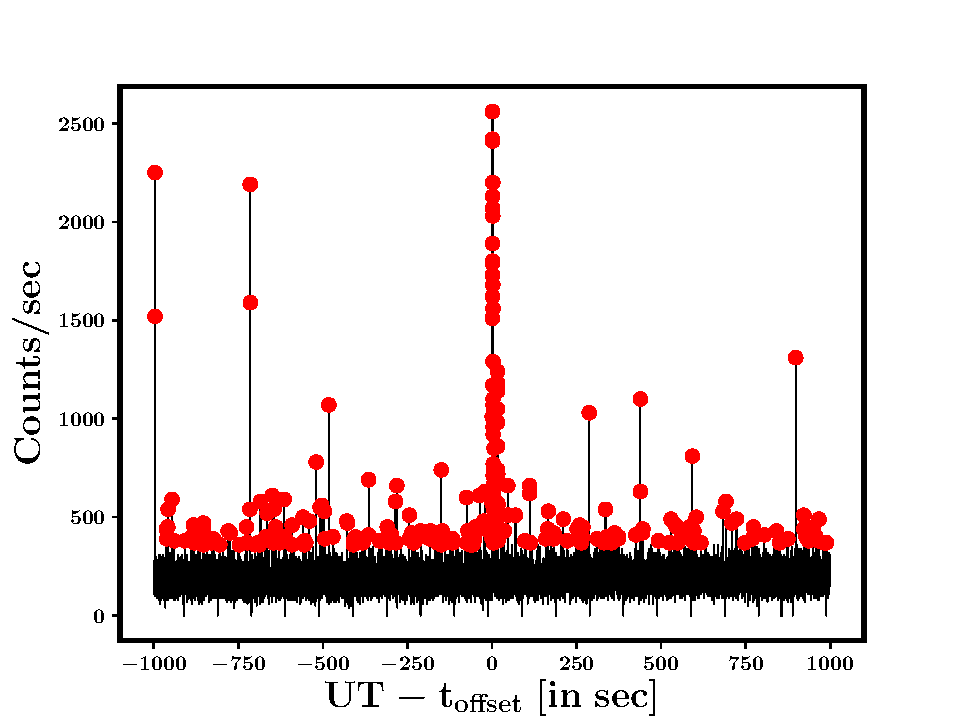
\includegraphics[scale=0.42]{GRB160802A--Q1--DPHclean_before}
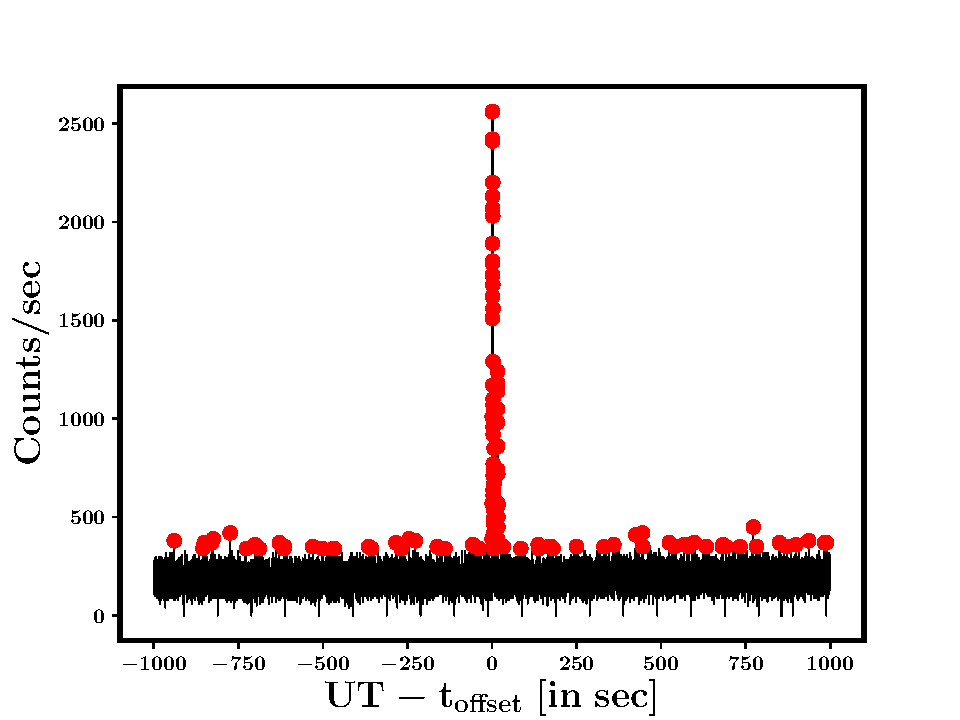
\includegraphics[scale=0.42]{GRB160802A--Q1--DPHclean_after}
\end{center}
\begin{center}
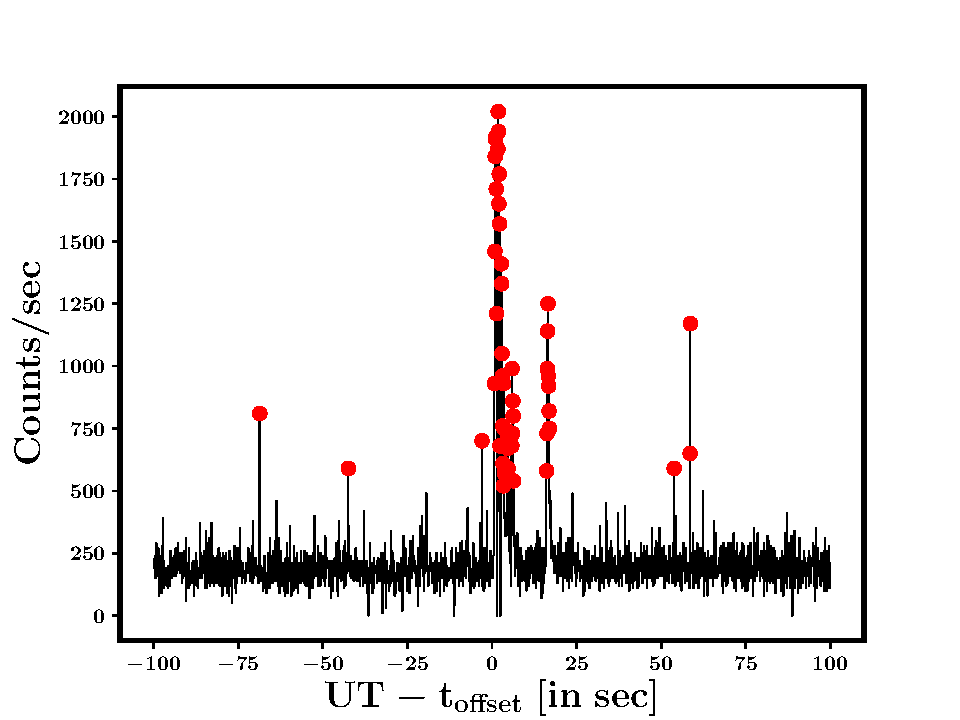
\includegraphics[scale=0.42]{GRB160802A--Q0--DPHclean_before--zoom}
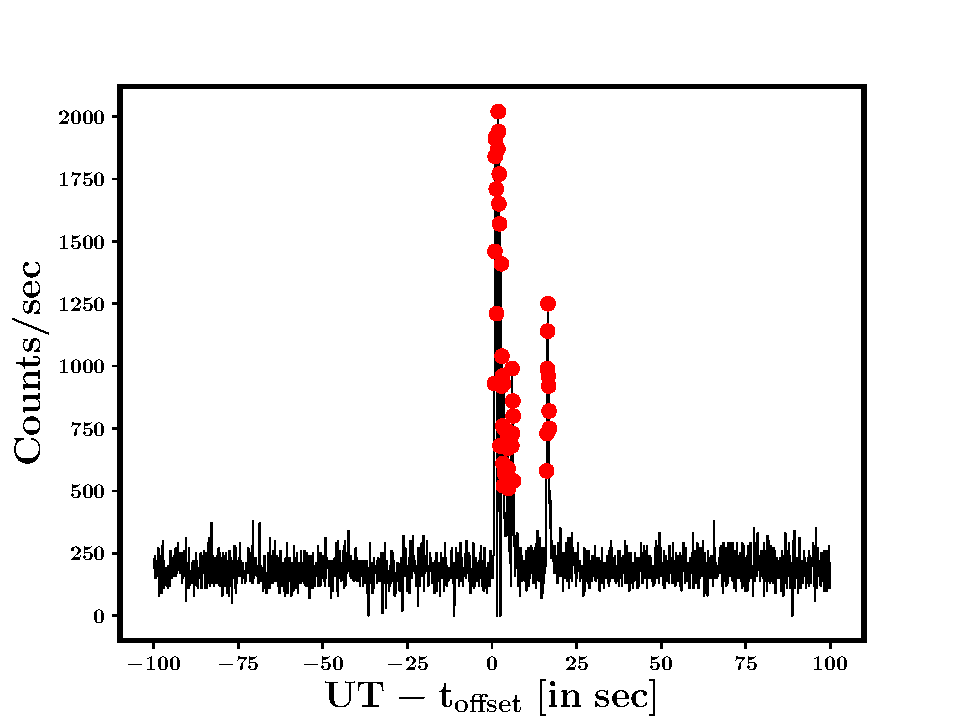
\includegraphics[scale=0.42]{GRB160802A--Q0--DPHclean_after--zoom}
\caption[The effect of DPHclean on the lightcurves of GRBs]{Lightcurves binned at $\tl = 100$ ms before [\eL] and after [\eR] DPHclean near the bright GRB160802A, red points showing $2 \sigma$ outliers. \emph{Top}: longer stretch of Q1; \emph{Bottom}: zoomed for Q0 [hence scale is different]. It is noted that sudden features in the lightcurve are removed by DPHclean, but GRB photons are not flagged. The second feature within $20$ seconds of the start of the prompt emission is also a part of the GRB, and is seen distinctly in the zoomed lightcurves of all quadrants with a similar profile, so it is not be mistaken as noise.}
\label{fig:GRB_zoom}
\end{center}
\end{figure}


\begin{figure}
\begin{center}
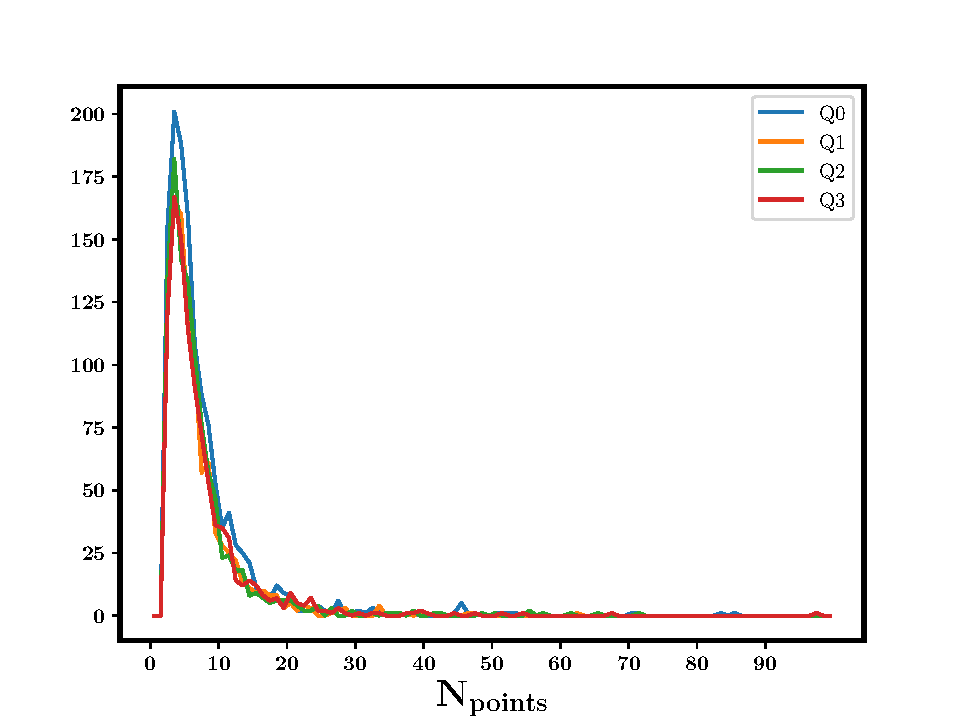
\includegraphics[scale=0.5]{Histogram_of_Npoints--observed}
\caption[Histogram of the number of unique points in the DPHstructures]{Histogram of the number of unique points in the DPHstructures.}
\label{fig:histogram_of_observed_Npoints}
\end{center}
\end{figure}



A large fraction of the events clustered in DPHstructures occupy regions only a few pixels wide, see Figure \ref{fig:histogram_of_observed_Npoints}. Some of these DPHstructures includes pixels which register counts $4$ or higher in $100$ ms bins. Here it is pointed out that in case a DPH shows clustering, only those events in the DPH that are responsible for the same are removed from the data by DPHclean. It that has the ability to identify them, and in the presence of such clustered events even during bright GRBs, the algorithm selectively picks out only the events in the cluster and removes them, instead of the GRB photons. The advantage of such selective identification is evident. It is noticed that running this algorithm on \emph{all} DPHs made from a given set of data reduces the noise significantly more than selectively running it on [say $5 \sigma$] outliers in the lightcurve. To highlight the case that randomly distributed GRB photons are left unharmed by DPHclean, Figure \ref{fig:GRB_zoom} compares the lightcurve binned at $\tl = 100$ ms before and after implementing this step.
%For the purpose of the pipeline flow, however, it is safe to remove all DPHstructure events.


\begin{figure}
\begin{center}
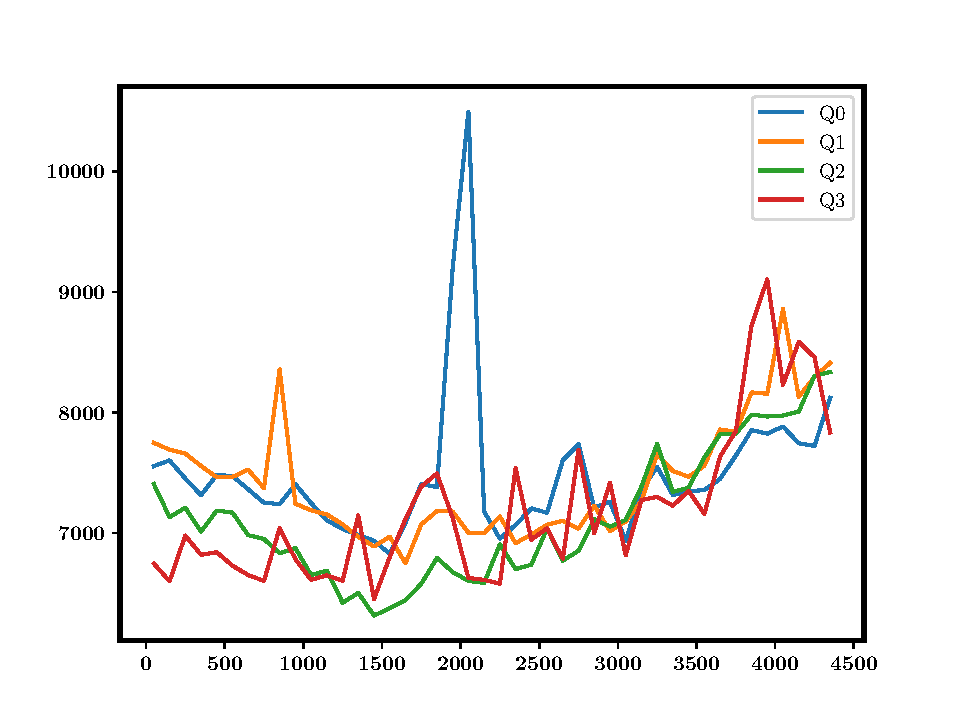
\includegraphics[scale=0.42]{LC_of_bunches}
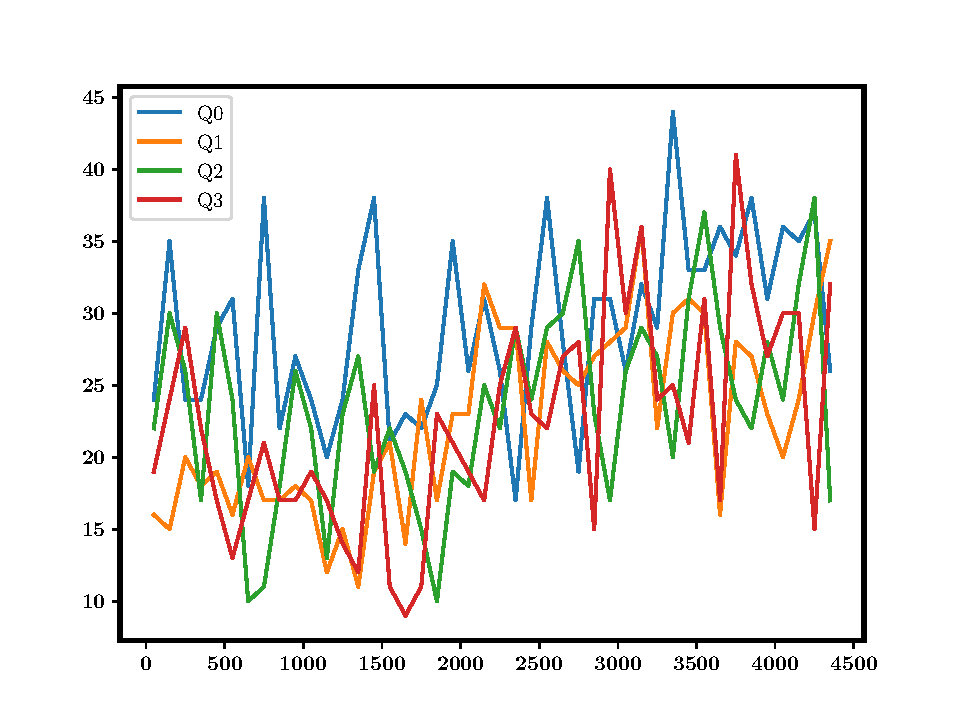
\includegraphics[scale=0.42]{LC_of_DPHstructures}
\caption[Lightcurves of bunches and DPHstructures for a full orbit data]{Lightcurves of bunches [\eL] and DPHstructures [\eR] binned at $ 100$ s, for a full orbit data. One of the quadrants [Q0] show a peak for the bunches, which is understood to be due to the rise of the number of bunches over several $1$ s intervals. However, such an increase is not seen for the same quadrant for the DPHstructures. The overall increase of the count-rate of both the bunches and the DPHstructures towards the end of the orbit as the satellite enters the SAA, indicates that both kind of events may be due to the common origin in charged particles.}
\label{fig:lightcurve_comparison_of_bunches_and_DPHstructures}
\end{center}
\end{figure}

\begin{figure}
\begin{center}
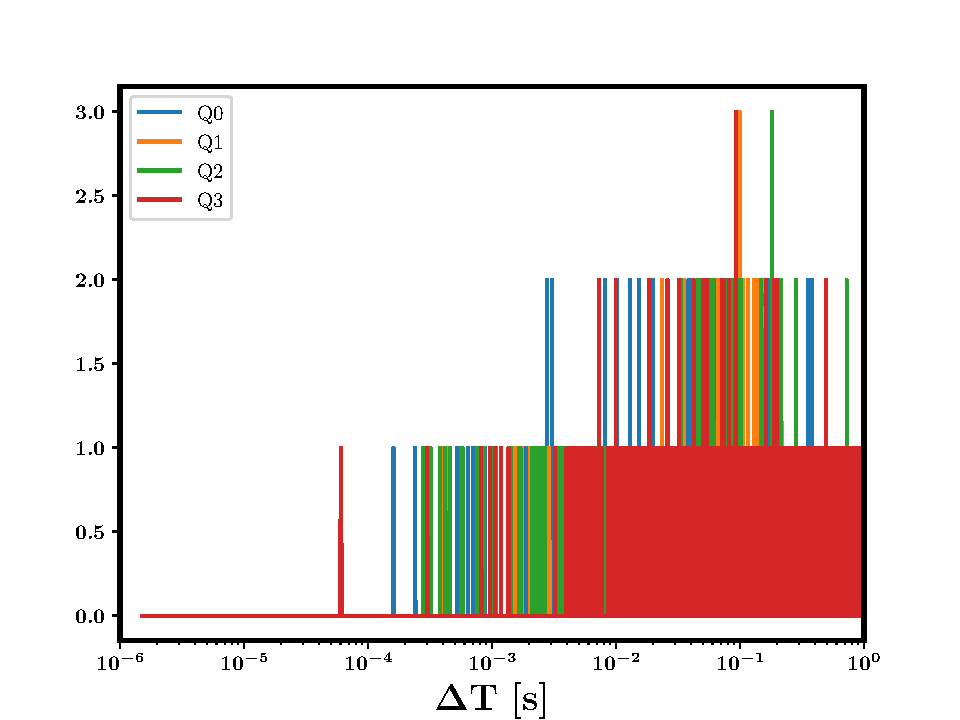
\includegraphics[scale=0.5]{delta_btn_DPHs_and_previous_bunch}
\caption[Histogram of the time difference between the start of a DPHstructure with the end of the bunch just preceding it]{Histogram of the time difference between the start of a DPHstructure with the end of the bunch just preceding it, denoted here as $\Delta T$. There is no non-statistical rise of the number of such coincidences all the way up to $\sim 100$ ms, indicating that there is no causal correlation between bunches and DPHstructures.}
\label{fig:correlation_between_bunches_and_DPHstructures}
\end{center}
\end{figure}


In  Figure \ref{fig:lightcurve_comparison_of_bunches_and_DPHstructures} are plotted the lightcurves of bunches and DPHstructures, both binned at $100$ s intervals for a full orbit data.  The overall rise towards the end of the orbit as the satellite enters the South Atlantic Anomaly [SAA] is clear for bunches, whereas for DPHstructures, it is only marginal. However, this similarity points to the origin of both kinds of events in charged particles. The quadrant-averaged orbit-averaged rate of DPHstructures is $0.245 \, \ps$.
%It is hypothesized that they are locally generated electronic noise or tails of cosmic ray bunches lingering in the data for timescales longer than bunches. On the other hand, it is most likely that the DPHstructures that cause strong outliers in lightcurves are caused by a physical mechanism that gives rise to genuine ionization in the detectors, and not random electronic noise.

We have investigated any possible temporal correlation of bunches with DPHstructures, to understand whether DPHstructures could be caused by heavy bunches. In Figure \ref{fig:correlation_between_bunches_and_DPHstructures} is shown the histogram of the difference between the start-time of a DPHstructure with the end-time of the bunch that just precedes it. No causality is found at time intervals less than $1$ ms. That is, bunches and individual DPHs are statistically independent events.
%This is concluded by rigorous investigation of the lightcurves of bunches and DPHstructures. The lightcurves of bunches with higher bunch-lengths are also considered for careful re-investigation, because being rarer than bunches of smaller lengths,  they may be due to higher energetic cosmic rays, thus falling in the continuum of the spectrum of the energy of the cosmic rays.


\cite{Segreto_et_al.-2003-A&A--INTEGRAL_cosmic_rays} [hereafter \citetalias{Segreto_et_al.-2003-A&A--INTEGRAL_cosmic_rays}] studied the detector characterisitics of the PICsIT detector plane on board INTEGRAL, and found events similar to DPHstructures. To investigate their cause, they plotted detector delay histograms [DDHs] corresponding to each DPHstructure. DDHs are histograms on the detector plane of the delay of the events contributing to a particular DPHstructure with respect to the first event. They found the evidence of two kinds of events: linear tracks, and a particular kind of delay pattern-- a gradual increase of the delay towards the centre of the ellipses that were illuminated. They explained these by the bombardment of the detector plane by charged particles or cosmic ray showers generated by hadronic and leptonic processes very close to the detector. They demonstrated that the delay in the first and last events in a particular DPHstructure being $\sim 100$ ms  could be explained by the saturation of the pixels by the extreme high energies of the charged particles, the pattern on the detector tracing the density of the cosmic ray showers in the logarithmic scale. Inspired by these findings, we plot DDHs for our DPHstructures, some examples are given in Figure \ref{fig:DDH}. We see two kinds of events:


\begin{enumerate}
\item Those tracing linear tracks indicating trajectories of physical entities along them [Figure \ref{fig:DDH}, \emph{Top}]. This points to the origin being charged particles which deposit their energy over multiple pixels that fall on its trajectory of motion through the detector.
\item Those with the delay being more in the inside of a cluster compared to its boundaries [Figure \ref{fig:DDH}, \emph{Bottom}].
\end{enumerate}

Both the kinds of events are in striking similarity with the DDHs observed in PICsIT on board INTEGRAL, and naturally leads one to the hypothesis that DPHstructures in CZTI are also created by the bombardment of high-energy charged particles or cosmic ray showers.

Some cosmic rays might deposit their energies over multiple pixels instead of a few because being more energetic than their counterparts that create bunches, they are above the detectable energy threshold of the pixels, thus saturating them. When the pixel output current drops below this threshold, they start registering events. The saturation timescale observed in the detectors then corresponds to the delay from the onset of the events created by these cosmic rays on the detector plane. The fact that DPHstructures are much less frequent than bunches, also corroborates such a hypothesis. Also, it naturally explains the delay pattern of the second kind, that is those with progressively higher delays towards the centre of the pattern \citepalias{Segreto_et_al.-2003-A&A--INTEGRAL_cosmic_rays}. When a cosmic ray shower hits the detector, the density of the particles in the shower are traced by the delay in the DDH. The delay timescale in the detector pixels are thus deduced to be a few $100$ milliseconds.


\begin{figure}
\begin{center}
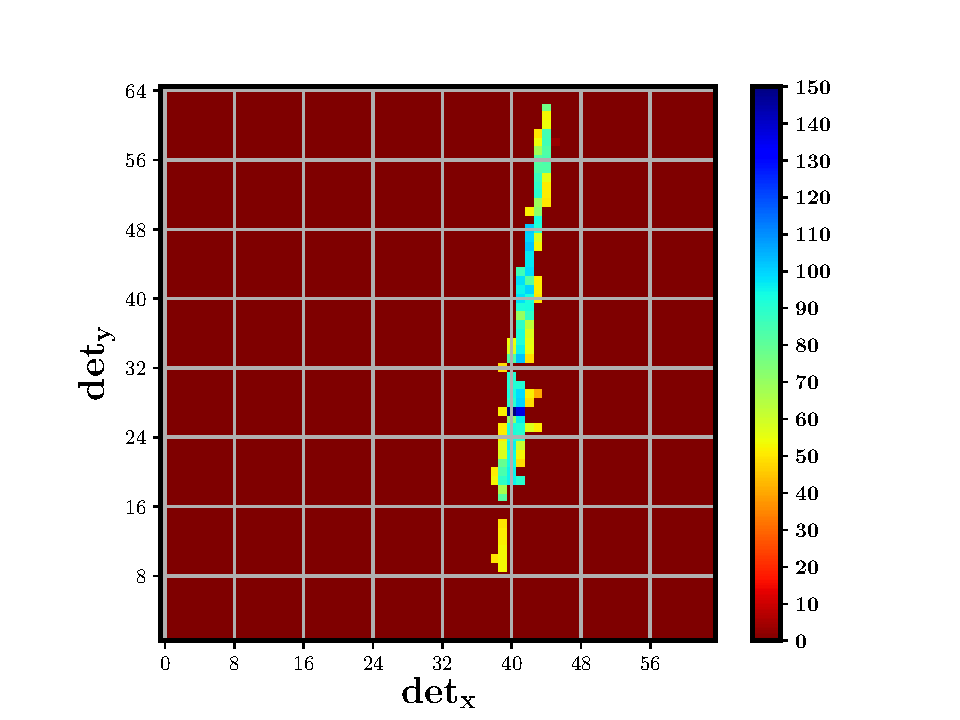
\includegraphics[scale=0.42]{Q1--merged_35+36}
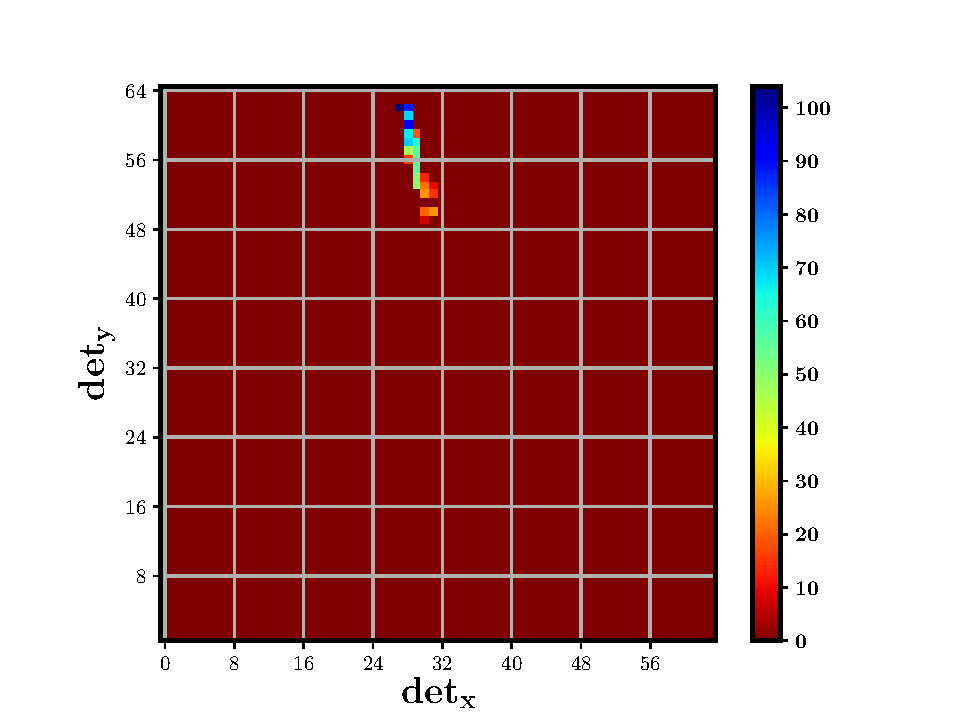
\includegraphics[scale=0.42]{Q1--merged_11114+11115}
\end{center}
\begin{center}
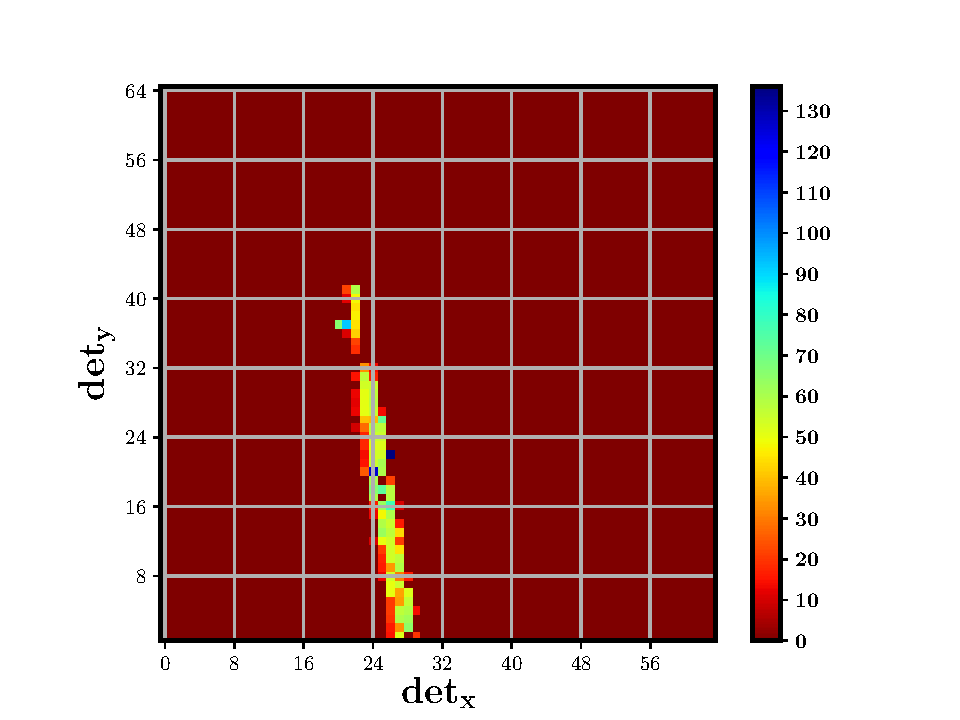
\includegraphics[scale=0.42]{Q1--merged_2853+2854}
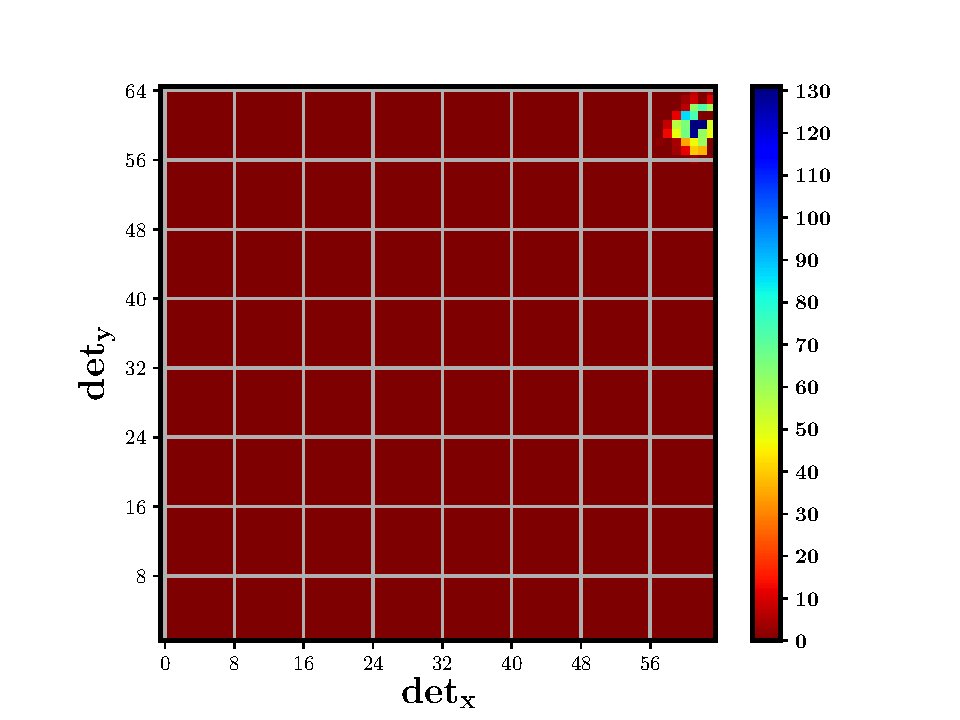
\includegraphics[scale=0.42]{Q3--merged_7861+7862}
\caption[Detector Delay Histograms showing patterns similar to INTEGRAL-PICsIT]{Detector Delay Histograms: Plotted in colour are the delay of the particular event from the first event in the cluster, in milliseconds, as a function of the position in the detector plane. These examples last unusually long, covering two consecutive bins. In \emph{Top}, we observe linear tracks, the delay increasing along the track in \emph{Top-Right}. The delay patterns in \emph{Bottom} are remarkably similar to those seen in PICsIT on INTEGRAL due to phosphorescence-decays from events triggered by cosmic ray showers.}
\label{fig:DDH}
\end{center}
\end{figure}


The energy of the cosmic rays cannot be calculated directly. However, we place constraints on the energy of both bunches and DPHstructures from the observed rate of the events, assuming a standard spectrum of cosmic rays \citepalias{Longair-3rd_Ed.}:

\begin{equation}
\frac{\dd N}{\dd E} =  1.8 \times 10^4 \rm{\dfrac{nucleons}{s \, m^2 \, sr \, GeV}} \left( \frac{E}{1 \, \rm{GeV}} \right)^{-2.7}.
\label{eq:cosmic_ray_spectrum}
\end{equation}

We assume that the DPHstructures illuminate $10$ pixels on an average, which is an area of $160 \, \rm{cm^2}$, and integrate over all solid angles, between energy limits $E_{\rm{min}}$ and $E_{\rm{max}}$ and match them with the observed rates of bunches and DPHstructures. For the purpose of continuity, we divide the DPHstructures into two kinds of events on the basis of their frequency, with the criterion being the number of unique points in the DPHstructure $\lessgtr 10$. The orbit-averaged, quadrant averaged, rates of bunches, high-frequency and low-frequency DPHstructures are respectively $70 \, \ps$, $0.200 \, \ps$, and $0.044 \, \ps$. Assuming an upper limit of the low-frequency DPHstructures as $100$ TeV, the energy-limits thus derived are shown in Figure \ref{fig:Energy_limits}. The lower limit of the bunch energies comes out to be $\sim 7$ GeV.


\begin{figure}
\begin{center}
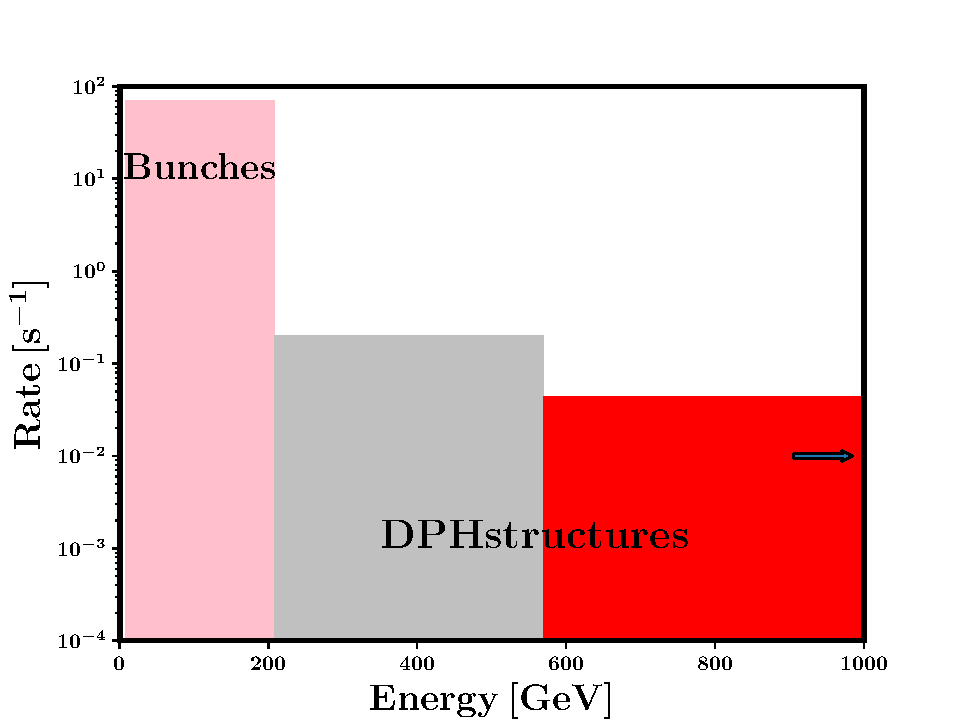
\includegraphics[scale=0.5]{Energy_limits}
\caption[Energy limits of bunches and DPHstructures]{The limits of the energies of three kinds of events: bunches, high-frequency DPHstructures, and low-frequency DPHstructures. The lower limit of the bunches is $ \sim 7 $ GeV. The frequency cut of DPHstructures is based on the number of unique points in the DPHstructures, and is put roughly at the start of the tail of this curve, see Figure \ref{fig:histogram_of_observed_Npoints}. The higher end of the low-frequency DPHstructures is $100$ TeV, but shown here only till $1$ TeV for representational purposes.}
\label{fig:Energy_limits}
\end{center}
\end{figure}


Finally, the question that remains unanswered is: What is the physical mechanism that creates the $\sim 100$ ms timescale saturation effect in the pixels? For PICsIT, the timescale was explained by fluorescence states of the CsI detectors, which is not possible for CdZnTe detectors of the CZTI. The only explanation is the following: The extreme high energy of the cosmic rays that hit the individual detectors lets current pass through the RC-circuit that provides stability to the source of power to these detectors. That is, due to the extremely high energy deposited in the individual detectors in an extremely small time, they successfully exchange power from the power source, thus remaining saturated until the impending RC-circuit has stabilized. Then the timescale of the saturation is given by the time-constant of the impending RC-circuit, which is $\sim 100$ ms. This is an interesting explanation to the question of how CZTI pixels get saturated with a $\sim 100$ ms timescale.


\section{Conclusions}
\label{sec:conclusions--noise}
The two tasks in the existing CZTI pipeline, the \textbf{cztbunchclean} and the \textbf{cztpixclean}, have been investigated thoroughly in this work, using data from multiple GRBs as test cases. Through careful investigation, a complete understanding of the effect of cosmic rays on CZTI data is presented. The term `noise' is understood rigorously, via patterns in the data that are representative of events definitely not triggered by astrophysical source photons, in this case GRB photons. Modifications to \textbf{cztbunchclean} are suggested. For \textbf{cztpixclean}, no modification to its first part involving the removal of data from grossly noisy pixels is required. However, a smarter and more robust algorithm called the `DPHclean' is suggested to replace the second part of this task, which currently involves the detection of temporarily flickering pixels by the average countrates as a function of time. The reason behind the flickering of pixels is identified to be higher energy cosmic rays that create predictable patterns on the detector plane, here called `DPHstructures'. The robustness of the algorithm is extensively demonstrated.

The optimized values of the parameters for the revised tasks in the pipeline are listed in Table \ref{tab:parameters}. `Livetime corrections' refer to the corrections to lightcurves due to the reduction of the exposure time of the detectors while cleaning the data of noise. Such corrections are initially calculated from L2 good time interval [GTI] data, updated sequentially after each step proposed, and implemented on the lightcurves. Livetime corrected lightcurves for a stretch of data before and after GRB160802A, at the start with L2 data, and after all steps of cleaning, are shown in Figure \ref{fig:cleaning_example}.%and \ref{fig:double_events}.


\begin{table}
\caption[Optimal values of the parameters in the improved pipeline]{Optimal values of chosen parameters in the proposed pipeline. $t_2$ and $t_3$ are discussed in Section \ref{sec:Bunchclean}, $\gc$ in Section \ref{sec:Gross_noisy_pixels}, $\tl$ in Section \ref{sec:DPHclean}, and $\thr$ and $\al$ in Appendix \ref{appendix:DPHstructures}.}
\label{tab:parameters}
\begin{center}
\begin{tabular}{|c|c|}
\hline 
Parameter & Proposed optimal values\\
\hline 
\hline 
$t_{2}$ & $60$ \\
\hline 
$t_{3}$ & $60 \, \mus$\\
\hline 
$\gc$ & $5$\\
\hline 
$\tl$ & $100$ ms\\
\hline 
$\thr$ & $0.70$\\
\hline 
$\al$ & $3$\\
\hline 
\end{tabular}
\end{center}
\end{table}


The current CZTI pipeline requires careful reprocessing of data of bright GRBs due to the conservative nature of the removal of `noise' from science data, which removes some GRB photons as well. This not only makes the continuum data before and after the GRBs more noisy, it also makes it currently impossible to independently search for GRBs in the wealth of CZTI data, limiting the searches to ones triggered by alerts from other space-based missions. Comparison of the number of GRBs detected by CZTI with such triggered searches, with predictions from the study of the luminosity function of GRBs, reveals that a good fraction of GRBs are yet to be found -- both the long \citep{Paul-2018-MNRAS--long} and the short \citep{Paul-2018-MNRAS--short} kinds. This requires development of an automated algorithm that searches for GRBs independently detected by CZTI. In this work, it is extensively demonstrated that the proposed modifications will segregate science data with noise in the same stead for continuum count-rates and bright GRBs, and have been developed keeping the natural durations of GRBs durations in mind. Thus, these modifications are a crucial precursor to an automated GRB-detection algorithm.


\begin{figure}
\begin{center}
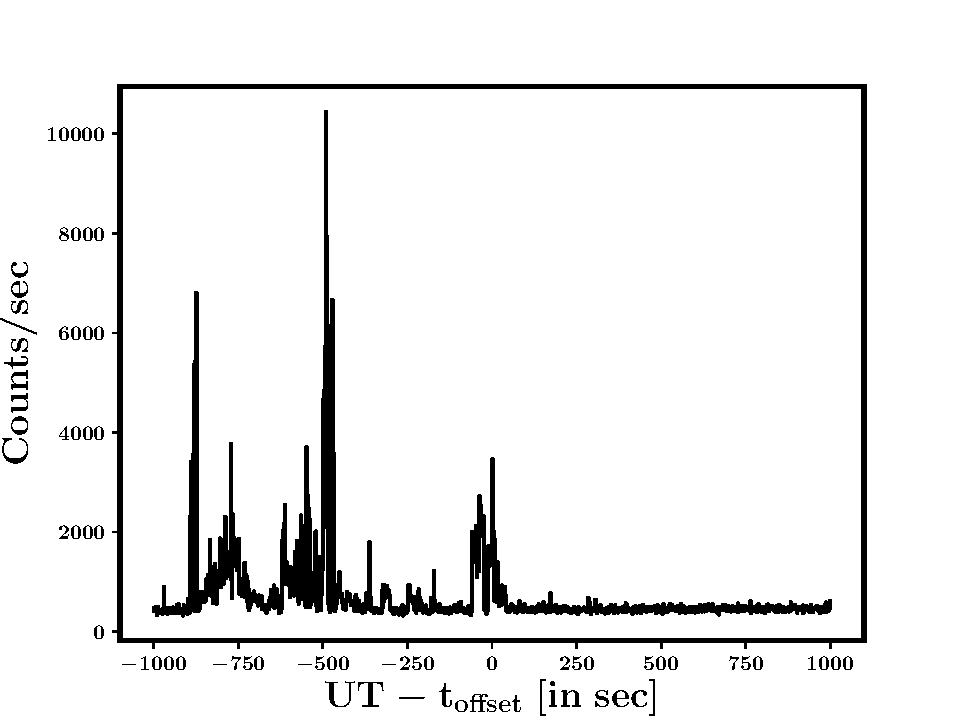
\includegraphics[scale=0.42]{GRB160802A--Q0--allevts_at_start--1s}
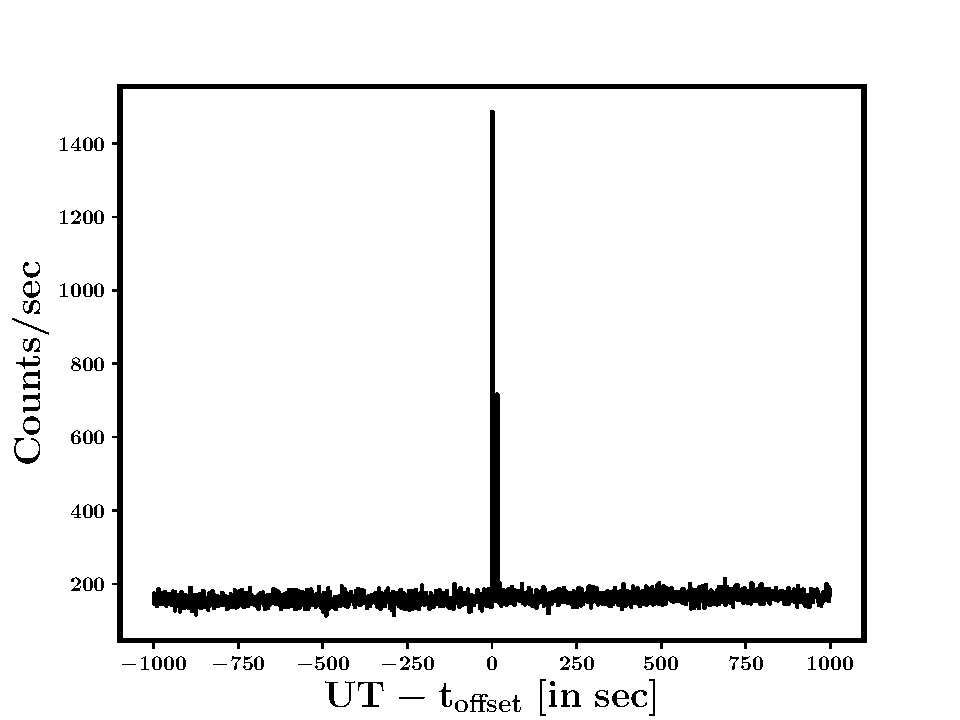
\includegraphics[scale=0.42]{GRB160802A--Q0--sglevts--cleaned_all--1s}
\caption[Lightcurves before and after data processing]{\eL: All events at start. \eR: All single events post cleaning.}
\label{fig:cleaning_example}
\end{center}
\end{figure}


%\begin{figure}
%\begin{center}
%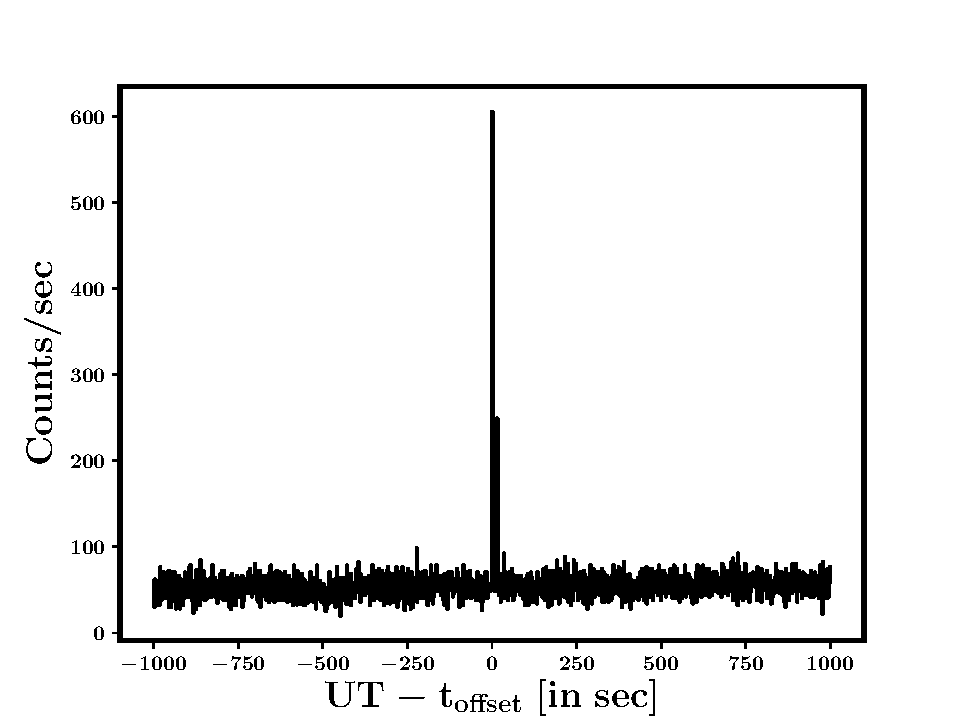
\includegraphics[scale=0.42]{GRB160802A--Q0--dblevts--cleaned_all--1s}
%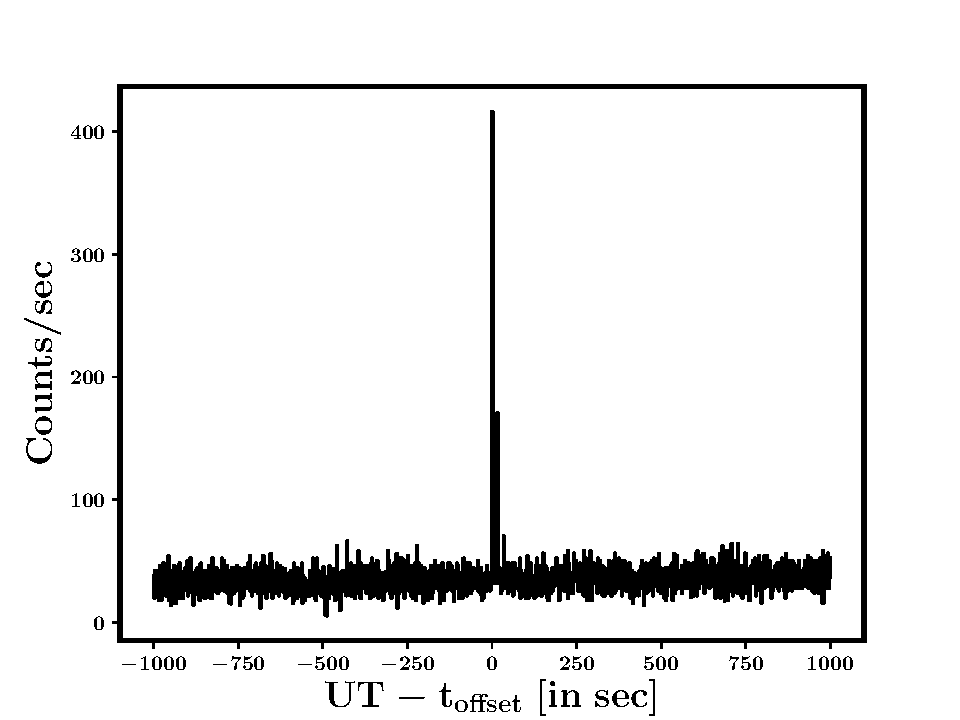
\includegraphics[scale=0.42]{GRB160802A--Q0--dblevts_roughCompton--cleaned_all--1s}
%\caption[Lightcurves of double events after data processing]{Double events post cleaning [includes all energies]. \eL: All double events. \eR: Only those exhibiting simple Compton criterion, i.e. those that are in neighbouring pixels only. The average of such rough Compton events is $30$ compared to $50$ for all double events, however the enhancement during the GRB appears comparable. The small discrepancy can be due to electronic effects of incident photons, as discussed in Section \ref{subsec:electronic_effects}.}
%\label{fig:double_events}
%\end{center}
%\end{figure}